\documentclass[10pt,a4paper,twocolumn]{article}
\usepackage[a4paper,margin=17mm,columnsep=6mm]{geometry}
\usepackage[T1]{fontenc}
\usepackage{newtxtext,newtxmath}
\usepackage{microtype}
\usepackage{amsmath}
\usepackage{booktabs}
\usepackage{graphicx}
\usepackage{xcolor}
\usepackage[font=small,labelfont=bf,skip=4pt]{caption}
\usepackage{enumitem}
\usepackage[hidelinks]{hyperref}
\usepackage{tabularx}
\usepackage{array}
\setlist{nosep,leftmargin=*}
\graphicspath{{fig/}}
\newcommand{\Tab}[1]{\input{tab/tab_#1.tex}}
\newcommand{\NAutoRod}{1918}
\newcommand{\NAutoV}{60}
\newcommand{\NClimbAtImpl}{5.3}
\newcommand{\NClimbAtImplMax}{5.9}
\newcommand{\NClimbAtImplMin}{4.5}
\newcommand{\NClimbHeavy}{7.0}
\newcommand{\NClimbLight}{10.7}
\newcommand{\NClimbVHeavy}{50}
\newcommand{\NClimbVLight}{60}
\newcommand{\NFailTthreeten}{1.0}
\newcommand{\NFailTtwoseventy}{2.4}
\newcommand{\NGeHundredKw}{363}
\newcommand{\NGeLowRatio}{0.89}
\newcommand{\NGovDroop}{0.28}
\newcommand{\NGovKwA}{367}
\newcommand{\NGovKwB}{487}
\newcommand{\NHovBank}{4.1}
\newcommand{\NHovIgeHeavy}{324}
\newcommand{\NHovIgeLight}{247}
\newcommand{\NHovLastAlt}{3658}
\newcommand{\NHovOgeHeavy}{364}
\newcommand{\NHovOgeLight}{275}
\newcommand{\NHovStallAlt}{4877}
\newcommand{\NHovStallCtHi}{0.12}
\newcommand{\NHovStallCtLo}{0.11}
\newcommand{\NImplAsIgeHeavy}{361}
\newcommand{\NImplAsOgeHeavy}{378}
\newcommand{\NImplMax}{378}
\newcommand{\NImplMean}{361}
\newcommand{\NImplMin}{342}
\newcommand{\NImplTdIgeHeavy}{342}
\newcommand{\NImplTdIgeLight}{300}
\newcommand{\NImplTdOgeHeavy}{365}
\newcommand{\NImplTdOgeLight}{286}
\newcommand{\NLock}{5.1}
\newcommand{\NLpHov}{$-$6.24}
\newcommand{\NLpHundred}{$-$4.22}
\newcommand{\NLpSixty}{$-$5.13}
\newcommand{\NMiAutoFpm}{1982}
\newcommand{\NMiAutoKt}{62}
\newcommand{\NMiAutoNrMin}{304}
\newcommand{\NMiCruiseKw}{332}
\newcommand{\NMiDuration}{419}
\newcommand{\NMiTouchFpm}{13}
\newcommand{\NMqHov}{$-$1.56}
\newcommand{\NMqHundred}{$-$2.33}
\newcommand{\NMqSixty}{$-$2.23}
\newcommand{\NNrHov}{$-$0.54}
\newcommand{\NNrHundred}{$-$1.47}
\newcommand{\NNrSixty}{$-$1.17}
\newcommand{\NPcruise}{326}
\newcommand{\NPhover}{364}
\newcommand{\NPmin}{224}
\newcommand{\NPtrimMax}{428}
\newcommand{\NPvne}{414}
\newcommand{\NSigma}{0.0607}
\newcommand{\NStEngaged}{83.2}
\newcommand{\NStIdleRpm}{16330}
\newcommand{\NStIdleTfour}{299}
\newcommand{\NStLightOff}{14.1}
\newcommand{\NStRotorNinetyFive}{81.7}
\newcommand{\NStRotorRpm}{20823}
\newcommand{\NStRotorTurns}{62.6}
\newcommand{\NStTfourRunup}{404}
\newcommand{\NStTfourStart}{384}
\newcommand{\NVh}{32.3}
\newcommand{\NVhFpm}{1940}
\newcommand{\NVmaxImpl}{197}
\newcommand{\NVmaxMcp}{112}
\newcommand{\NVmaxMcpKmh}{208}
\newcommand{\NVmin}{60}
\newcommand{\NVrsTenHi}{2501}
\newcommand{\NVrsTenLo}{939}
\newcommand{\NVrsTenZhi}{1.29}
\newcommand{\NVrsTenZlo}{0.48}
\newcommand{\NVrsZeroHi}{2819}
\newcommand{\NVrsZeroLo}{869}
\newcommand{\NVrsZeroZhi}{1.45}
\newcommand{\NVrsZeroZlo}{0.45}
\newcommand{\NVtip}{204}
\newcommand{\NVtrimMax}{115}
\newcommand{\NVtrimMaxLight}{125}
\newcommand{\NZwHov}{$-$0.34}
\newcommand{\NZwHundred}{$-$0.90}
\newcommand{\NZwSixty}{$-$0.81}
\newcommand{\NnFcs}{256}
\newcommand{\NnFunc}{581}
\newcommand{\NuFlap}{1.017}
\newcommand{\NuLag}{0.183}

\newcommand{\ok}{\textcolor{green!45!black}{\ensuremath{\checkmark}}}
\newcommand{\nok}{\textcolor{red!70!black}{\ensuremath{\times}}}
\newcommand{\pok}{\textcolor{orange!85!black}{\ensuremath{\sim}}}
\renewcommand{\arraystretch}{1.08}
\setlength{\tabcolsep}{4pt}
\raggedbottom
\renewcommand{\topfraction}{0.92}\renewcommand{\dbltopfraction}{0.92}\renewcommand{\bottomfraction}{0.6}
\renewcommand{\textfraction}{0.06}\renewcommand{\floatpagefraction}{0.85}\renewcommand{\dblfloatpagefraction}{0.85}
\setcounter{topnumber}{3}\setcounter{dbltopnumber}{3}\setcounter{totalnumber}{5}
\makeatletter\setlength{\@fptop}{0pt}\setlength{\@dblfptop}{0pt}\makeatother
\begin{document}

\twocolumn[
\begin{@twocolumnfalse}
\begin{center}
{\LARGE\bfseries Flight Dynamics of the Sud Aviation SA 316B Alouette III in JSBSim\par}
\vspace{6pt}
{\large\bfseries An articulated-rotor blade-element model with a single-shaft turboshaft, built from public data and flown through a scripted test programme\par}
\vspace{10pt}
{\large Technical report \quad\textbullet\quad November 2026\par}
\vspace{10pt}
\end{center}
\begin{abstract}
\noindent
A flight-dynamics model of the Alouette III for the FlightGear simulator has been written in JSBSim, replacing the model built on
JSBSim's generic rotor that the aircraft flew before. Its fully articulated rotor is simulated blade by blade: three rigid blades on
coincident flap and lag hinges (the lag frequency \NuLag{} per revolution), with a viscous lag damper, eight segments each on tables of its
NACA 63A011.5 section built from Boeing Vertol's C-81 equations for the 0012 and like-for-like wind tunnel data, under a Peters--He finite-state wake with Johnson's vortex ring model, ground effect and a
ring-vortex wake on the tail surfaces. The Turbomeca Artouste III B is modelled as what it is, a single-shaft engine whose spool is
geared to the rotor through a centrifugal clutch and a freewheel, with its isochronous governor, its starter and its inertia. Since the
Alouette's rotor turns clockwise, the aerodynamics are worked in the aircraft's mirror image. The model, \NnFunc{} aerodynamic functions and
\NnFcs{} control-system components, is generated from transcribed data and runs in plain JSBSim at 480\,Hz. No flight-test time histories
of the Alouette III are public, so the scripted programme checks what can be checked: the published performance, the published
start, the rotor's physics against theory, and a test flight flown by an autopilot from lift-off to touchdown. The model hovers at
2200\,kg on \NPhover\,kW and reaches the 405\,kW continuous rating at \NVmaxMcpKmh\,km/h against the published maximum of 210\,km/h. The
published hover ceilings imply that only \NImplMin--\NImplMax\,kW reach the rotor, and at that power the model climbs at
\NClimbAtImplMin--\NClimbAtImplMax\,m/s against the published 4.3--5.5\,m/s: the published performance is consistent with itself and
with the model only at about nine-tenths of the rated power, a discrepancy left open rather than tuned away. The start runs as published
(idle at \NStIdleRpm\,rpm against 15\,000--18\,000, the rotor taken up at \NStRotorRpm\,rpm of the engine against 19\,500--21\,000), and in vertical descent the heave
mode is unstable from \NVrsZeroLo{} to \NVrsZeroHi\,ft/min, the vortex ring state.
\end{abstract}
\vspace{6pt}
\end{@twocolumnfalse}
]

% =====================================================================================================================
\section{Introduction}
The Alouette III distributed for FlightGear (by G.\ Robin and others, with later systems work) is a detailed aircraft: cockpit, systems,
a hoist, a co-pilot who hovers for it. Its flight model used JSBSim's built-in rotor, which computes a rotor's thrust and moments
from a few parameters in closed form; it flew, but not like a helicopter of the Alouette's kind. The Alouette III is a light utility
helicopter of 1959: a fully articulated three-bladed rotor turning clockwise seen from above (the French practice), a three-bladed
tail rotor on the right of an open lattice boom, and a single-shaft Turbomeca Artouste turboshaft whose compressor and turbine turn at
constant speed and drive the rotor through a centrifugal clutch.

Unlike the Bo 105 and UH-60A, whose models this one follows and which had flight tests and full analysis decks to be checked against, the
Alouette III has no published flight-test time histories, identified derivatives or blade structural data. What is public is its type
certificate, the engine's, performance figures in several sources (which disagree), a few technical papers, a fuselage wind tunnel
test, tyre data, and descriptions of the start of its sister, the Lama (Table~\ref{tab:sources}). This report describes a model built on that,
after the Bo 105 and UH-60 models, and a test programme that checks it where the data allow; where they do not, it says so. All result
tables, figures and the numbers quoted from them are written by the evaluation scripts.

% =====================================================================================================================
\section{Reference data}\label{sec:ref}
\begin{table}[t]
\centering\small
\caption{Sources and what they contribute.}\label{tab:sources}
\begin{tabularx}{\columnwidth}{@{}>{\raggedright\arraybackslash}p{2.3cm}X@{}}
\toprule
Source & Content used \\
\midrule
EASA TCDS R.123~\cite{tc} & dimensions, rotor speeds and limits, masses, CG range and datum, fuel, transmission limits, $V_{NE}$ \\
EASA TCDS E.091~\cite{te} & Artouste III B: stages, speeds, ratings, T4 limits, reduction gear, mass \\
This Day in Aviation~\cite{td} & rotor senses and speeds, tail rotor; speeds, hover ceilings, climb at 2200 and 1750\,kg \\
A\'erostories~\cite{as} & specification table of the Artouste version: speeds, climb, hover and service ceilings, range \\
heli-archive.ch \cite{ha} & rotor and engine description; the gearbox-limited power held to 4000--4500\,m; fuel flow \\
2nd ERF~\cite{e76} & the rotor head's mass \\
3rd ERF~\cite{e77} & the Artouste's isochronous governor and automatic start \\
14th ERF~\cite{e88} & the Alouette II's metal blade: mass, chord, section, twist \\
20th ERF~\cite{e94} & the Alouette III fuselage in the wind tunnel: lift and drag against angle of attack \\
Michelin, Goodyear~\cite{mi} & the 355$\times$150-4 tyres: loads, deflection, sizes \\
ROTORwrench \cite{rw} & the Lama's Artouste IIIB1: idle, the starter's cut-out \\
Lama add-on manual~\cite{lm} & a flight simulator's, after the flight manual: the engine speed at which the rotor turns, the rotor brake \\
HAL description~\cite{hl} & a licence-built SA 316B: blade chord, section and twist, lag dampers, tail rotor sections, fuel burn \\
RST 1/2020~\cite{rs} & the blade's chord along the span, after the pilot's handbook \\
TR 75-50~\cite{c81} & C-81's NACA 0012 equations, the sections' base \\
NACA 903, 824~\cite{n903,n824} & the 63A010 and 63$_1$-012 in the Langley tunnel; critical Mach numbers \\
NASA TM 4074~\cite{tm4074} & the 0012 in the same tunnel, smooth and rough \\
NACA 460~\cite{n460} & the 0012, 0015 and 0018: slopes, maximum lift, minimum drag \\
Sound recordings & the tail rotor's gearing, from its blade-passing frequency; the start's pace, idle, the clutch's slip \\
AOPA Pilot, 1972~\cite{ao} & a flight test of an SE 3160: autorotative descent, idle, the clutch \\
FlightGear 3-D model & hinge offset, blade span and chord, tail surfaces, wheels, lights \\
Johnson~\cite{johnson} & the vortex ring state model \\
NASA TN D-234~\cite{heyson} & ground effect in forward flight \\
\bottomrule
\end{tabularx}
\end{table}

A few points of data reduction matter for the comparisons.
\emph{(i)} The sources' performance figures disagree. At 2200\,kg This Day in Aviation gives hover ceilings of 1650\,m in ground effect and 100\,m
out of it, A\'erostories 2850 and 1100\,m; the cruise speed is 180, 185 or 195\,km/h. All are read as sea level, standard day.
\emph{(ii)} The blade's mass and inertia are not published. The Alouette II's metal blade, of the same construction, weighs 28.9\,kg for 4250\,mm
of span and 280\,mm of chord~\cite{e88}; scaled to the Alouette III's span and chord it gives 38.7\,kg, a Lock number of \NLock.
\emph{(iii)} The blade's twist, 6$^\circ$30$'$, and its section, NACA 63A of 11.5\,\% thickness, are Hindustan
Aeronautics' description of the type~\cite{hl}, which names no camber: the section is taken as the symmetrical 63A011.5. The tail
rotor's sections are NACA 0015 to 0018, taken as 0018 at the root and 0015 at the tip. No full tables of these sections, over the
whole circle and up to the advancing tip's Mach number, are published; they are built from C-81's 0012 (Section~\ref{sec:sections}).
\emph{(iv)} The hinge offset, the blades' aerodynamic span and the tail surfaces come from the FlightGear 3-D model, whose blade animation
pivots on the hinges.
\emph{(v)} The control ranges are not published: the type certificate refers to the maintenance manual for the rigging. They
are estimates wide enough to trim from the hover to beyond $V_{NE}$.

% =====================================================================================================================
\section{The model}\label{sec:model}
\subsection{Implementation}
A Python script writes the model from the transcribed data (Table~\ref{tab:model}). JSBSim evaluates aerodynamic functions on demand, so
the function graph must be free of cycles; every quantity that depends on its own past (the blades' flap and lag angles and rates, the
rotor's azimuth and speed, the wake states, the tail rotor's flapping and inflow, the engine's spool, fuel and temperature) lives in
control-system channels, integrated explicitly. The model runs at 480\,Hz, 4.4$^\circ$ of the rotor's azimuth and 24.2$^\circ$ of the tail rotor's per step; the airframe's loads,
the engine and the outputs at 240\,Hz, the original aircraft's systems (electrics, lights, gauges, its autopilot) at 120\,Hz. The
report's programme run at 960\,Hz gives the same numbers, to within 1\,\% or their last digit, but for the start's clutch, which
engages 0.7\,s sooner at 480, and the last trim at 1750\,kg, 5\,kt further on the stall's edge; 400\,Hz still holds them, while at 360 the clutch's run-up changes and at 320 the stopped rotor's friction no longer holds it. The rotor turns clockwise seen from above and the tail rotor sits on the right, pushing left: the
mirror image of the UH-60's and Bo 105's layouts, whose rotor equations the generator shares. The aerodynamics are therefore worked in
the aircraft's mirror image across its plane of symmetry (the lateral velocity, the roll and yaw rates and their accelerations, the
lateral acceleration and the bank angle negated), and the side force, rolling and yawing moments negated back.

\begin{table}[t]
\centering\small
\caption{The generated model: JSBSim system files.}\label{tab:model}
\Tab{model}
\end{table}

\begin{table}[t]
\centering\small
\caption{Main data (TC type certificate, TD This Day in Aviation, TE engine certificate, E88 14th ERF, AC a blade, VP Vertipedia,
HL Hindustan Aeronautics' description, SR sound recordings' blade-passing frequencies, 3D the FlightGear 3-D model).}\label{tab:params}
\Tab{params}
\end{table}

\subsection{Main rotor}
The three blades are rigid, on coincident flap and lag hinges \NuFlap{} and \NuLag{} per revolution in flap and lag
(Table~\ref{tab:params}), with the UH-60 model's flap and lag equations: the aerodynamic moments, the blade's weight and the hub's
specific force, the gyroscopic and Coriolis terms, the centrifugal stiffness through the hinge offset, and the airframe's angular
velocity and acceleration. A viscous lag damper gives 25\,\% of critical damping at the rotor's speed (an estimate); flap, droop and lag
stops limit the blades. Each blade, twisted 6.5$^\circ$~\cite{hl}, has eight segments of equal annulus area outboard of its root, on the
tables of its NACA 63A011.5 section (Section~\ref{sec:sections}) at the segment's angle of attack and Mach number, with a drag
increment of 0.0012 for a production blade and a 3\,\% tip loss.
The hub's forces and moments come from the blades' loads at the hinges, their inertial reactions included, at the hub's position in the
airframe. The rotor's speed is solved together with the three lag accelerations, as in the Bo 105 model: the blades' lag and the hub
exchange angular momentum through the hinges.

\subsection{Inflow and wake}
The Peters--He finite-state wake has five states (four cosine harmonics, one sine), driven by the blades' segment lifts, with a time
constant that follows the mass flow. In descent the mass flow parameter is Johnson's~\cite{johnson}, as in the MV-22B model: through the
vortex ring state the induced velocity rises above momentum theory's and the rotor loses thrust at a fixed collective, the heave mode
going unstable. Ground effect scales the induced velocity with the hub's height as the Bo 105 and UH-60 models do, with Heyson's ratio
into forward flight~\cite{heyson}; its strength is theirs, not fitted. A ring-vortex model of the main rotor's wake, precomputed against
skew angle and the stations' positions, gives the downwash at the tail rotor, the stabiliser, the end plates, the fuselage and the boom.

\subsection{Tail rotor}
The three-bladed tail rotor is a blade-element rotor with six segments per blade on NACA 0018 (root) to 0015 (tip) tables, each blade on its own flapping
hinge, with the 5$^\circ$ toe of its hub (3-D model) and a Pitt--Peters inflow. It is geared 5.487:1 to the main rotor, the ratio of
the two rotors' blade-passing frequencies in seven recordings of governed Alouette III and Lama rotors, so that it turns at 1938\,rpm.
The published 2001\,rpm~\cite{td,hl} is the tail rotor's speed at a main rotor's of about 365\,rpm: Hindustan Aeronautics pairs it with
363\,rpm~\cite{hl}, a ratio of 5.51, while the 353.2\,rpm it is usually quoted with would make 5.67.

\subsection{Blade sections}\label{sec:sections}
The sections' tables start from C-81's 0012 equations~\cite{c81} (lift slope and maximum lift against Mach number, the drag
polynomial and its rise, the flat plate past the stall, reversed flow) and take the differences that like-for-like tests give. In the
Langley low-turbulence pressure tunnel the 0012~\cite{tm4074}, the 63A010~\cite{n903} and the 63$_1$-012~\cite{n824} were measured
smooth and with standard roughness (6A and 6-series sections of one thickness have the same maximum lift and drag~\cite{n903}). The
C-81 0012 lies between the smooth and the rough 0012: its maximum lift at Mach 0.15, 1.36, is two thirds of the way from the rough
section's to the smooth one's at 3~million Reynolds number, the retreating blade's when it stalls, and its zero-lift drag with the
production increment, 0.0092, nearly the rough section's at 6~million, the hovering and advancing blade's. The 63A011.5, interpolated
in thickness, is placed the same way between its own smooth and rough values; the 0012 gains maximum lift with Reynolds number and the
63A hardly any. Its tables thus take 0.91 of the 0012's maximum lift up to Mach 0.3, going to the 0012's at Mach 0.6, where both
sections' stall is the shock's and their critical Mach numbers at high lift are about the same~\cite{n824} (an estimate: no high-speed
data of a 63A section were found); add 0.0026 of drag at a lift of 0.6, growing with the angle of attack squared; and move the drag
divergence Mach number up by 0.028, the difference of the two sections' critical Mach numbers at zero lift~\cite{n824}, fading out by
3.7$^\circ$, where their curves meet. The lift-curve slopes are the same, 0.107 per degree. The tail rotor's 0015 and 0018 take their
slopes, maximum lifts and minimum drags relative to the 0012 from the variable-density tunnel's series~\cite{n460} (drag 12 and
30\,\% higher, maximum lift the same and 3\,\% lower), and their drag divergence 0.040 and 0.075 earlier, the 63-series' change of
critical Mach number with thickness~\cite{n824}.

\subsection{Airframe}
The fuselage's lift and drag against angle of attack are the 20th ERF's wind tunnel data for the Alouette III~\cite{e94}, on the rotor
disc's 95\,m$^2$; side force and yawing moment by the cross-flow principle, with the body's Munk moments. The parts the tests leave out
(the open tail boom, the gear, the rotor head and mast, and the rest) are cross-flow and flat-plate estimates; the last, 4\,ft$^2$, is a
round figure, not fitted. The stabiliser (0.8\,m$^2$ between its end plates) and the end plates are lifting surfaces in the rotor's wake.

\subsection{Flight controls}
Collective, cyclic and pedals drive the swashplate and the tail rotor's pitch through hydraulic servos (the UH-60's response, for want of the
Alouette's), with no augmentation. FlightGear's trims shift the controls' centres. The original aircraft's autopilot (heading and altitude
holds) and its co-pilot for the hoist add to the pilot's controls, as they did before.

\subsection{Engine, drive and mass}
The Artouste III B is a single-shaft turboshaft: its compressor and turbine turn at 33\,500\,rpm, 94.85 times the rotor's speed, at whatever
power~\cite{te,e77}. Its hydromechanical governor is modelled as an isochronous PI controller on the spool's speed, its fuel limited by the
turbine temperature (T4, 550\,$^\circ$C at the thermal maximum). The spool's torque comes from the fuel beyond what it needs to turn
unloaded; the thermal maximum, 640\,kW at sea level, lapses with altitude so that the gearbox's 420\,kW is held to 4250\,m~\cite{ha}.
The start follows the published descriptions~\cite{rw,lm} and, in its pace, two recorded starts: the starter cranks the spool,
its torque falling to nothing at 17\,\% as an electric starter's, the spool at 10\,\% in 4\,s; the start system's fixed fuel flow
until idle; light-off at 16\,\%, about 14\,s after the starter, which goes off line at 14\,000\,rpm; idle at 16\,330\,rpm (a cockpit
recording's; about 15\,000~\cite{ao}, and 17\,000--18\,000 for the Lama's engine~\cite{rw}) about 30\,s after light-off, with the fuel
flow lever at 35\,\%. Advancing the lever, the centrifugal clutch slips
from 19\,000\,rpm~\cite{ao} with its shoes' sliding friction, fitted to the recordings' take-ups (the rotor from rest at flat pitch,
the spool held): about 1150\,ft\,lb at the rotor at 62\,\% of the spool's speed and 1490 at 80\,\%, so that the rotor locks to
a spool at 80\,\% in 44\,s (45 recorded) and at 61\,\% in 62\,s (64 at 63\,\%), and above as a centrifugal clutch's, with the
speed squared. Locked, its capacity, full by 24\,000\,rpm, carries any flight torque. A freewheel lets the rotor overrun the engine. The
spool's inertia, 0.15\,kg\,m$^2$, is 1350\,kg\,m$^2$ at the rotor's speed, as much as the rotor's own, added to it once the clutch has
locked: half the drive's. The rotor brake and the transmission's breakaway friction hold the rotor at rest. The mass and CG are the type's, with the
loads at their stations and a fuel tank that burns down.

\subsection{Landing gear}
Three 355$\times$150-4 tyres~\cite{mi}: their spring rates from the static deflection at the rated load, the nose wheel castoring.

\subsection{FlightGear}
The original aircraft's cockpit and systems (electrical, instruments, autopilot, co-pilot, crash detection, animations) stay; a bridge
system maps them onto this model's properties. An in-air start holds the airframe for its first seconds while four loops trim the
collective and FlightGear's trims on the vertical and angular accelerations, through the inverse of the model's control Jacobian, before
letting go; the aircraft starts with its trimmed bank. For FlightGear's HDR pipeline the exterior lights are spot lights with halos.

% =====================================================================================================================
\section{Method}\label{sec:method}
The model is flown offline in JSBSim's Python interface at 480\,Hz. Trims solve for collective, cyclic, pedals, pitch attitude and bank (or
sideslip) by Newton iteration with the airframe held and the rotor running, on the body accelerations averaged over two revolutions with a
Hann window once the rotor and its wake have settled; with the rotor speed held at 353.2\,rpm the engine's power is the drive's load: main
and tail rotors, gearbox losses and accessories. Climbs and autorotations are trims along a sloping flight path, solved for the angle at
which that power equals the power available, or nothing. Derivatives are central differences of the held airframe's loads.

A test autopilot, the UH-60 model's adapted, flies what trims cannot. It holds wheel height, ground velocity and heading in the hover;
altitude, airspeed, heading by bank and sideslip in forward flight; and the rotor's speed with the collective in autorotation. Its inner
loops damp the aircraft on its rates, since the Alouette has no augmentation, at crossovers chosen from the control powers. On the wheels
it raises the collective steadily with the cyclic and pedals following it as a pilot's would, holds the brakes, and lets its attitude and
heading loops take over once the wheels carry less than a fifth of the weight; it lowers the collective after touchdown. The same
autopilot is a FlightGear autopilot of the aircraft.

% =====================================================================================================================
\section{Results}\label{sec:results}
\subsection{Level-flight trim and performance}\label{sec:trims}
\begin{figure*}[t]
\centering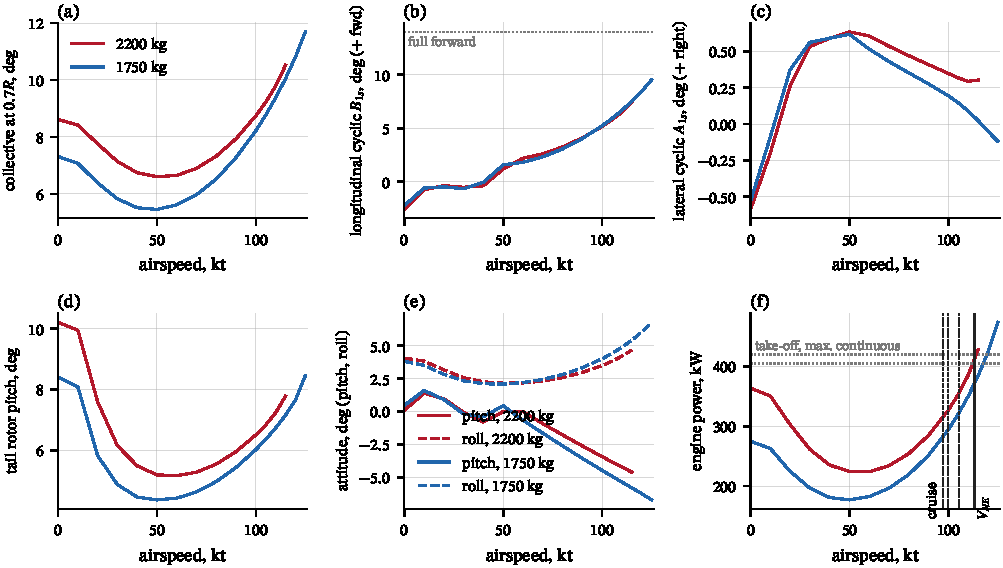
\includegraphics[width=\textwidth]{trims.pdf}
\caption{Level-flight trims at sea level, 2200 and 1750\,kg: (a)--(d) controls, (e) attitudes, (f) the engine's power against the ratings,
with the published cruise speeds (dashed) and $V_{NE}$.}\label{fig:trims}
\end{figure*}
\begin{table*}[t]
\centering\small
\caption{Performance against the published figures (AS A\'erostories, TD This Day in Aviation, AO the AOPA Pilot's flight test~\cite{ao}). At the published hover ceilings, the model's power to hover there:
the power available that each ceiling implies.}\label{tab:perf}
\Tab{perf}
\end{table*}
Figure~\ref{fig:trims} shows the trims. At 2200\,kg the model hovers out of ground effect on \NPhover\,kW and needs least, \NPmin\,kW,
at \NVmin\,kt; the bank is \NHovBank$^\circ$ right in the hover, the tail rotor's push balanced. It reaches the 405\,kW continuous rating at
\NVmaxMcpKmh\,km/h, against 210\,km/h published as the maximum speed and $V_{NE}$. Past 100\,kt the power rises steeply, and the
last trim is at \NVtrimMax\,kt (\NPtrimMax\,kW; \NVtrimMaxLight\,kt at 1750\,kg): beyond it the retreating blades stall, the
63A section's lower maximum lift setting the type's speed limit about where its $V_{NE}$ is. The longitudinal cyclic keeps a margin to
its stop.

Table~\ref{tab:perf} sets the model against the published figures. The airframe's drag is reasonable (at 100\,kt an equivalent flat
plate of 1.4\,m$^2$), but the performance is not: with the rated power the model would hover out of ground effect far higher than either
source and climb faster. Read the other way, the power to hover at each published ceiling is the power available that ceiling implies:
\NImplMin--\NImplMax\,kW, against the 405--420\,kW ratings. At that power the model climbs at \NClimbAtImplMin--\NClimbAtImplMax\,m/s,
the published 4.3--5.5\,m/s, and its maximum level speed is \NVmaxImpl\,km/h, the published cruise speeds. The published figures are thus
consistent with one another and with the model at about nine-tenths of the rated power: either less power reaches the Alouette's rotor
than the ratings say, or the real rotor and airframe need a fifth more power than the model. Which, the public data do not tell; the
model is left at the ratings and its rotor untuned, and a user who wants the published performance in FlightGear would reduce the
power available, not the rotor's efficiency.

\subsection{The hover and ground effect}\label{sec:hover}
\begin{figure}[t]
\centering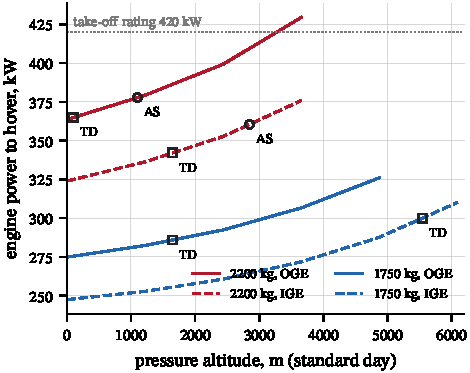
\includegraphics[width=\columnwidth]{hover.pdf}
\caption{Power to hover against altitude, in ground effect (1\,m wheel height) and out of it, with the published ceilings placed on the
model's curves (AS circles, TD squares).}\label{fig:hover}
\end{figure}
\begin{figure}[t]
\centering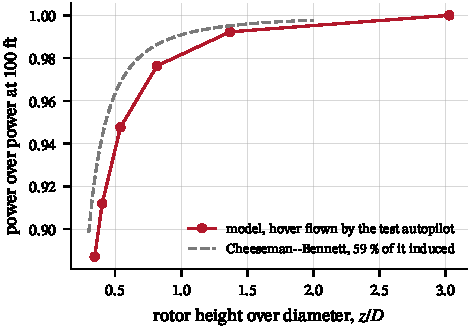
\includegraphics[width=\columnwidth]{ge.pdf}
\caption{Ground effect: the power to hover flown by the test autopilot at each wheel height, over the power at 100\,ft, against
Cheeseman and Bennett's ground effect on the induced share of the power (the weight times the hover's induced velocity).}\label{fig:ge}
\end{figure}
Figure~\ref{fig:hover} shows the power to hover against altitude. At 2200\,kg the hover out of ground effect can no longer be trimmed at
\NHovStallAlt\,m (it can at \NHovLastAlt\,m): the blades reach the 63A section's stall ($C_T/\sigma$ between \NHovStallCtLo{} and
\NHovStallCtHi) before the power runs out, so even at the
ratings the model's ceiling there is its rotor's. Figure~\ref{fig:ge} shows ground effect as the test autopilot flew it:
lifting off, then holding 3, 5, 10, 20, 40 and 100\,ft of wheel height for half a minute each, steady to a few hundredths of a foot. At
3\,ft the hover needs \NGeLowRatio{} of the power at 100\,ft (\NGeHundredKw\,kW). Each source's ceilings in ground effect imply less
power available than its ceilings out of it (A\'erostories \NImplAsIgeHeavy{} against \NImplAsOgeHeavy\,kW, This Day in Aviation
\NImplTdIgeHeavy{} against \NImplTdOgeHeavy\,kW, at 1\,m of wheel height): either their hover in ground effect is higher than a metre, or
the model's ground effect, the Bo 105's and UH-60's strength and not fitted, is somewhat strong for the Alouette.
\begin{table}[t]
\centering\small
\caption{Ground effect flown by the test autopilot, 2200\,kg, sea level.}\label{tab:ge}
\Tab{ge}
\end{table}

\subsection{Climb and autorotation}\label{sec:climb}
\begin{figure}[t]
\centering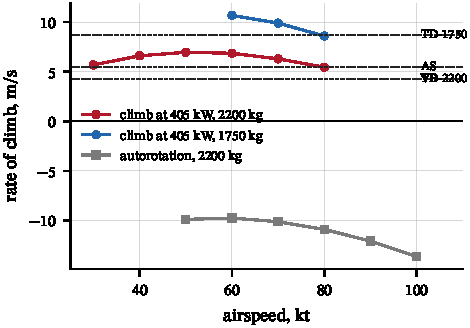
\includegraphics[width=\columnwidth]{climb.pdf}
\caption{Rate of climb at the maximum continuous power, and steady autorotation with the rotor at 353\,rpm, 1000\,ft; the published climb
rates dashed.}\label{fig:climb}
\end{figure}
With the 405\,kW continuous rating the model climbs at \NClimbHeavy\,m/s at 2200\,kg (\NClimbVHeavy\,kt) and \NClimbLight\,m/s at
1750\,kg (Fig.~\ref{fig:climb}), against 4.3--5.5 and 8.7\,m/s published: the excess power of the previous section again. In steady
autorotation the rate of descent is least, \NAutoRod\,ft/min, at \NAutoV\,kt.

\subsection{A test flight}\label{sec:mission}
\begin{figure*}[t]
\centering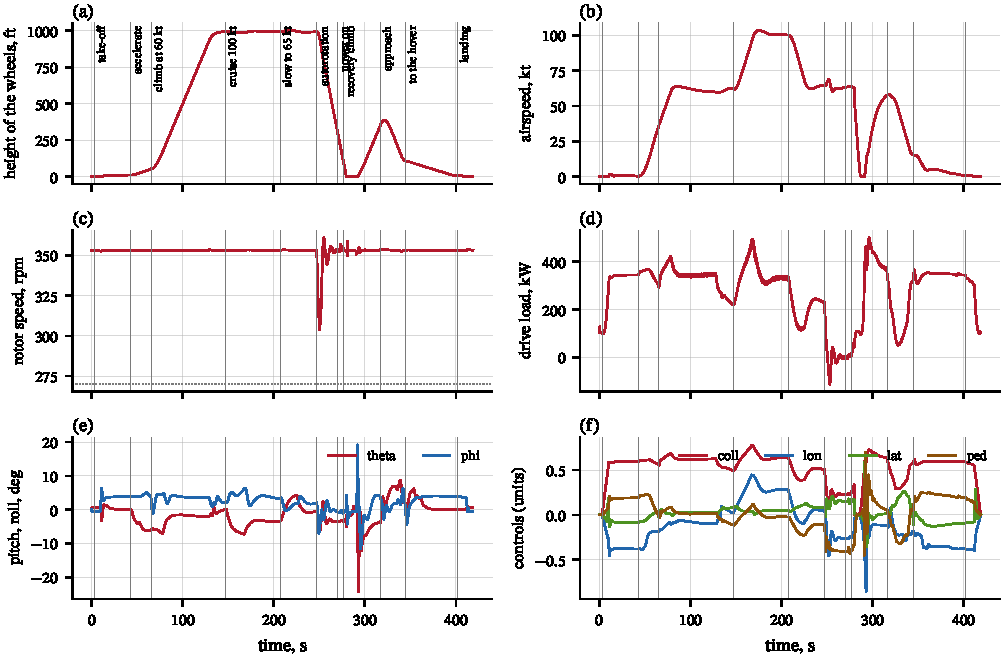
\includegraphics[width=\textwidth]{mission.pdf}
\caption{A test flight flown by the test autopilot, 2200\,kg: take-off to a 10\,ft hover, acceleration, climb to 1000\,ft at 60\,kt,
cruise at 100\,kt, a practice autorotation at 65\,kt with the fuel flow lever at idle, power recovery, approach, hover, landing. The
drive's load is the engine's power while the clutch is engaged; in autorotation the rotor drives the tail rotor and the gearbox itself.}\label{fig:mission}
\end{figure*}
Figure~\ref{fig:mission} is a complete flight of \NMiDuration\,s, flown by the test autopilot from the wheels to the wheels. In cruise at
100\,kt the engine gives \NMiCruiseKw\,kW. For the practice autorotation the fuel flow lever goes to idle: the engine runs down to
\NStIdleRpm\,rpm, the freewheel lets the rotor overrun it, and the autopilot lowers the collective to hold the rotor's speed, which sags to
\NMiAutoNrMin\,rpm at the entry, as it would with a pilot's two-second reaction, and recovers. The steady descent at \NMiAutoKt\,kt is
\NMiAutoFpm\,ft/min. With the lever back to flight the engine accelerates, the freewheel takes up the drive as the spool catches the rotor,
and only then does the autopilot climb, as a pilot waits for the needles to join. It lands at \NMiTouchFpm\,ft/min.

\subsection{Derivatives, modes and step responses}\label{sec:derivs}
\begin{table}[t]
\centering\small
\caption{Derivatives at 2200\,kg, 1000\,ft (SI, per rad; controls per \% of travel), and the modes.}\label{tab:derivs}
\Tab{derivs}\\[4pt]
\Tab{modes}
\end{table}
\begin{figure*}[t]
\centering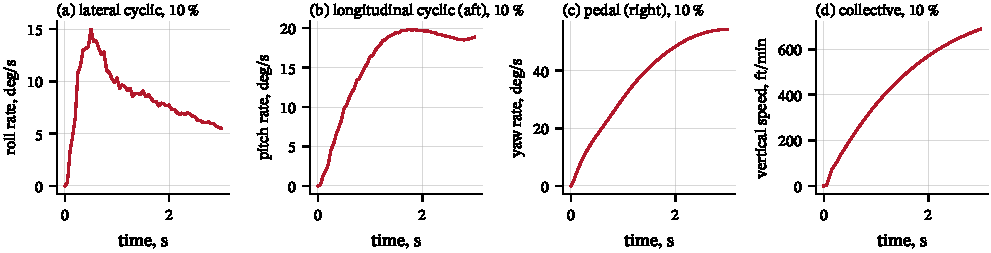
\includegraphics[width=\textwidth]{steps.pdf}
\caption{Responses of the free aircraft in the hover (2200\,kg, out of ground effect) to 10\,\% of each control's travel, held.}\label{fig:steps}
\end{figure*}
No identified derivatives of the Alouette III are public; Table~\ref{tab:derivs} lists the model's. They are those of an articulated
rotor with a small hinge offset under a light, narrow airframe. The roll damping $L_p$ is \NLpHov\,s$^{-1}$ in the hover, high for its
class because the roll inertia is small; the pitch damping $M_q$, \NMqHov\,s$^{-1}$, is a quarter of it, the pitch inertia being nearly five
times larger. The yaw damping $N_r$ is \NNrHov\,s$^{-1}$ and the heave damping $Z_w$ \NZwHov\,s$^{-1}$. The hover's modes are the classic
unaugmented helicopter's: a short-period roll subsidence and a slow, unstable pitch--speed oscillation. Figure~\ref{fig:steps} shows the
responses to steps: the roll rate peaks within half a second and then falls away as the aircraft starts to slide sideways and its
dihedral effect resists; the pitch rate builds more slowly and keeps building for two seconds, as the articulated rotor's lower pitch
damping lets it; the yaw rate builds over three, against little yaw damping.

\subsection{The start, the governor, a power failure}\label{sec:engine}
\begin{figure*}[t]
\centering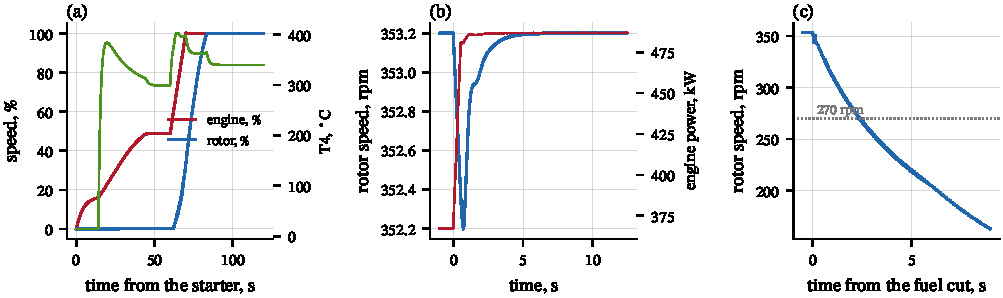
\includegraphics[width=\textwidth]{engine.pdf}
\caption{(a) The start: the starter pressed at 0\,s, the fuel flow lever advanced from idle over 10\,s at 60\,s; (b) the governor, the
collective raised 10\,\% of its travel in 0.5\,s in the hover; (c) a power failure at 60\,kt, the collective held.}\label{fig:engine}
\end{figure*}
The start (Fig.~\ref{fig:engine}a) runs as described~\cite{rw,lm}. The engine lights off at \NStLightOff\,s, the starter drops out at
14\,000\,rpm and it idles at \NStIdleRpm\,rpm (15\,000--18\,000~\cite{ao,rw}) and \NStIdleTfour\,$^\circ$C; T4 peaks at \NStTfourStart\,$^\circ$C in the start, under the
630\,$^\circ$C limit. With the lever advanced the rotor starts turning at \NStRotorRpm\,rpm of the engine (19\,500--21\,000 in the
add-on's manual~\cite{lm}), the clutch locks \NStEngaged\,s after the button and the rotor is at 95\,\% at \NStRotorNinetyFive\,s (the lever here goes to full
in 10\,s, the spool governed while the clutch still slips; held at the recordings' 80\,\%, the rotor locks to it 44\,s after it
starts turning, and the spool and rotor then reach governed speed together as fast as the lever goes); T4 peaks at
\NStTfourRunup\,$^\circ$C as the engine carries the rotor up. Raising the collective 10\,\% in the hover, the power rises from \NGovKwA{}
to \NGovKwB\,kW and the rotor droops \NGovDroop\,\%: the single-shaft engine is the rotor's flywheel, and its governor has no droop of its
own. With the power gone at 60\,kt and the collective held, the rotor falls below 310\,rpm in \NFailTthreeten\,s and to the 270\,rpm limit
in \NFailTtwoseventy\,s, the time a pilot has to lower the collective.

\subsection{The vortex ring state}\label{sec:vrs}
\begin{figure*}[t]
\centering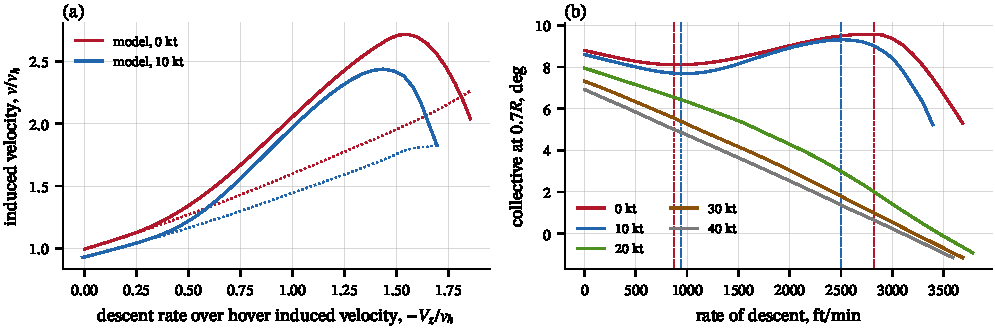
\includegraphics[width=\textwidth]{vrs.pdf}
\caption{Steady descents at 2200\,kg, 1000\,ft: (a) the induced velocity against the descent rate, model (solid) and momentum theory
(dotted), in vertical descent and at 10\,kt; (b) the collective against the descent rate at each speed, where it turns the heave mode's
stability boundary (dashed).}\label{fig:vrs}
\end{figure*}
In descent the induced velocity follows Johnson's model (Fig.~\ref{fig:vrs}). The hover's induced velocity is \NVh\,ft/s
(\NVhFpm\,ft/min). In vertical descent the collective needed falls with the descent rate down to \NVrsZeroLo\,ft/min and rises beyond it
to \NVrsZeroHi\,ft/min: between the two, more descent needs more collective, so at a fixed collective the descent runs away, the vortex
ring state's settling. At 10\,kt the region is \NVrsTenLo--\NVrsTenHi\,ft/min; from 20\,kt, where the edgewise flow exceeds the induced
velocity, there is none.

% =====================================================================================================================
\section{Corrections found during the test programme}\label{sec:review}
\begin{itemize}
\item \emph{The in-air start.} FlightGear trims an aircraft that starts in the air with JSBSim's own trim, which cannot trim this rotor:
the aircraft dived away. Holding the airframe while four loops trimmed the controls, at gains guessed from the control powers, let it go
untrimmed: the model's control powers were three to four times the guesses, and the loops hunted. They now use the inverse of the
model's control Jacobian and converge in two seconds; and since FlightGear starts the aircraft wings level, the aircraft supplies its
trimmed bank.
\item \emph{The rotor at rest.} With the friction at standstill a smooth function of the rotor's speed and the speed floored at zero, the
blades' swing on their hinges could ratchet a parked rotor round. A static friction now holds it while the torque from outside the
rotor, from the clutch, the engine or the air, is less than the brake's and the transmission's.
\item \emph{The clutch.} As it locked, the spool's inertia entered the rotor's equation a step late: for that step the rotor's
acceleration had the hub's inertia alone, a hundredth of the drive's, and the torque it put on the airframe, several hundred thousand
ft\,lb, yawed the aircraft on its wheels; the clutch then let go and locked again. Slipping, it passed its whole capacity at any slip,
and the hub, light with its blades free in lag, chattered about the spool's speed. The spool's inertia now follows the clutch's state,
the shaft's torque is taken before the state changes, and the slipping clutch's torque rises over 2\,rad/s of slip.
\item \emph{The electrical master} was off after an in-air start: lights and instruments had no power.
\item \emph{The test scripts} placed the aircraft on the ground at a CG height read before the model had computed its mass properties,
a foot or more low; the test autopilot's wheel height had the same error.
\item \emph{The lift-off.} The UH-60's autopilot lifted the Alouette level with the hover's lateral cyclic: its tail rotor's push to the
left, balanced in the hover by the thrust's lean to the right, rolled it over its left wheel within a foot. Its cyclic now comes in as
the aircraft gets light, as a pilot's does, with the stick aft, the Alouette's CG being ahead of its mast.
\item \emph{Fitted parameters.} The model's comments claimed that ground effect, the miscellaneous drag and the engine's lapse were fitted
to the published performance; none was, and they now say what they are.
\end{itemize}

% =====================================================================================================================
\section{Assessment}\label{sec:assess}
\begin{table}[t]
\centering\small
\caption{Summary: \ok{} reproduced, \pok{} partly or by construction, \nok{} not reproduced, -- no data to check.}\label{tab:score}
\begin{tabularx}{\columnwidth}{@{}>{\raggedright\arraybackslash}Xc@{}}
\toprule
Hover, climb and speed performance at the rated power & \nok \\
The published performance with one another, at \NImplMin--\NImplMax\,kW & \ok \\
Airframe drag (wind tunnel fuselage) & \pok \\
The start: idle, the clutch's engagement & \ok \\
Rotor speed limits in autorotation & \pok \\
Ground effect & \pok \\
Vortex ring state (Johnson's model) & \pok \\
Trim controls and attitudes & -- \\
Derivatives, modes, responses & -- \\
\bottomrule
\end{tabularx}
\end{table}
Table~\ref{tab:score} summarises. Where the Alouette III's published data reach, the model agrees with them in its engine's behaviour and,
at about nine-tenths of the rated power, in its performance; at the rated power it outperforms the aircraft, an open question whose
answer lies outside the public data. Its dynamics rest on physics and on estimates (the blades' mass and inertia, the lag damper, the
control ranges, the servos) for which no Alouette data are public, and nothing published checks the trims, the derivatives or the
responses. The model is flown well by an autopilot with a pilot's technique, which says that it handles like a helicopter; whether it
handles like this helicopter, only an Alouette pilot can say.

% =====================================================================================================================
\section{Conclusions}\label{sec:concl}
\begin{itemize}
\item A blade-by-blade model of the Alouette III's articulated rotor, with a finite-state wake, Johnson's vortex ring state, a
blade-element tail rotor, the wind-tunnel fuselage and a single-shaft Artouste with its clutch, freewheel, governor, starter and inertia,
runs in plain JSBSim, generated from public data. It is the flight model of the FlightGear Alouette III.
\item Its rotor turns the Alouette's way, through a mirror-image formulation of the UH-60 and Bo 105 models' equations.
\item The start, idle and the clutch's engagement follow a recording, the AOPA Pilot's flight test, a maintenance description of the
Lama's engine and a simulator manual after the Lama's flight manual; the Alouette III's own flight manual was not at hand.
\item The published performance is consistent with itself and with the model at \NImplMin--\NImplMax\,kW; at the 405--420\,kW ratings the
model hovers higher and climbs faster than any source gives. The discrepancy is documented, not tuned away.
\item A test autopilot flies the model from lift-off through cruise and a practice autorotation to touchdown.
\end{itemize}

\begin{thebibliography}{99}\small
\bibitem{tc} European Union Aviation Safety Agency, \emph{Type-Certificate Data Sheet EASA.R.123, SE 3130, SE 313, SA 3180, SA 318, SE 3160, SA 316, SA 319}, issue 3, 2017.
\bibitem{te} European Union Aviation Safety Agency, \emph{Type-Certificate Data Sheet EASA.E.091, Artouste III}, issue 3, 2024.
\bibitem{td} ``Sud-Aviation SA 316B Alouette III'', \emph{This Day in Aviation}, after A\'erospatiale's data.
\bibitem{as} ``SE 3160 Alouette III'', \emph{A\'erostories}.
\bibitem{ha} ``SE 3160 Alouette III'', \emph{heli-archive.ch}.
\bibitem{e76} A\'erospatiale, \emph{Design philosophy for helicopter rotor heads}, 2nd European Rotorcraft Forum, 1976.
\bibitem{e77} Turbom\'eca, \emph{Engine regulation}, 3rd European Rotorcraft Forum, 1977.
\bibitem{e88} \emph{Eight years of flight operations with composite rotor blades}, 14th European Rotorcraft Forum, 1988.
\bibitem{e94} \emph{Preliminary three-dimensional CFD model of a helicopter fuselage}, 20th European Rotorcraft Forum, 1994.
\bibitem{mi} Michelin, \emph{Aircraft Tire Engineering Data}; Goodyear, \emph{Global Aviation Tires} data book.
\bibitem{rw} S.\ Skola, ``ROTORwrench: Tips, Tricks and Info'', \emph{JustHelicopters}, November 2017 (the SA 315B Lama's Artouste IIIB1).
\bibitem{lm} \emph{SA 315B Lama}, user manual of a flight simulator add-on, 2023; its procedures follow the type's flight manual.
\bibitem{hl} Hindustan Aeronautics, technical description of an SA 316B Alouette III (1976), as quoted in the aircraft's sale listing.
\bibitem{rs} ``Aerodynamic analysis of Alouette III rotary wings'', \emph{Review of the Air Force Academy}, 1/2020, pp.\ 45--53.
\bibitem{ao} R.\,W.\ Sweazey, ``Pilot Flight Check: Alouette III'', \emph{The AOPA Pilot}, October 1972.
\bibitem{c81} Boeing Vertol Company, \emph{Validation of Rotorcraft Flight Simulation Program through Correlation with Flight Data for Soft-in-Plane Hingeless Rotors}, USAAMRDL TR 75-50, 1976 (the C-81 airfoil equations for the 0012).
\bibitem{n903} L.\,K.\ Loftin, \emph{Theoretical and Experimental Data for a Number of NACA 6A-Series Airfoil Sections}, NACA Report 903, 1948.
\bibitem{n824} I.\,H.\ Abbott, A.\,E.\ von Doenhoff, L.\,S.\ Stivers, \emph{Summary of Airfoil Data}, NACA Report 824, 1945.
\bibitem{tm4074} C.\,L.\ Ladson, \emph{Effects of Independent Variation of Mach and Reynolds Numbers on the Low-Speed Aerodynamic Characteristics of the NACA 0012 Airfoil Section}, NASA TM 4074, 1988.
\bibitem{n460} E.\,N.\ Jacobs, K.\,E.\ Ward, R.\,M.\ Pinkerton, \emph{The Characteristics of 78 Related Airfoil Sections from Tests in the Variable-Density Wind Tunnel}, NACA Report 460, 1933.
\bibitem{johnson} W.\ Johnson, \emph{Model for Vortex Ring State Influence on Rotorcraft Flight Dynamics}, NASA TP-2005-213477, 2005.
\bibitem{heyson} H.\,H.\ Heyson, \emph{Ground Effect for Lifting Rotors in Forward Flight}, NASA TN D-234, 1960.
\bibitem{jsbsim} JSBSim Development Team, \emph{JSBSim: an open-source flight dynamics model}, version 1.3.3.
\end{thebibliography}
\end{document}
